\chapter{Discussion} \label{sec:discussion}
In this chapter we will discuss aspects of this project which could have been done differently whether it being a result of making a decision to excluding something, choosing one approach over another, or simplifications.

\subsection*{Iterative Adjustment of the Nanosatellite Configuration} \label{subsec:disc_itt}
Iterative adjustment of the nanosatellite configuration was never implemented. We estimated that it was not possible to make a correct and non naive implementation within the given time frame of this project.

The downside of having the user to manually adjust their configuration is that they have to decide on which parts of the input that have to be tuned. An automatic process could be able to analyse the schedule for bottlenecks or other parts that would be candidates for change. It can be difficult process to manually find the variables that may lead to schedule that is not possible, or not robust\jfx{Hvad forsoeger vi at sige her?}. They are also limited in what the are able to change, as it is not possible to modify all of the internal variables. Some are hidden anyway to lower the required knowledge of the internal tools, UPPAAL \gls{cora} and \gls{smc}, in order to make the system easier to use\jfx{skulle vi som minimum ikke have inkluderet dem i vores global config fil, sa useren havde mulighed for at styre sa mange af variablerne som de kan?}. 
%Instead of having to manually adjust the configuration, it could be possible to make the system self configurable at the end of an iteration. Either to explorer new schedules or a more aggressive robustness analysis. For example, \cref{fig:tool_act}  have added an additional step to the tool-chain by allowing the system to loop if the robustness queries were unsatisfied. The system would then have to adjust the variables, such as the [min, max]

Since the iterative adjustment of the nanosatellite configuration have become manual, we have supplied an updated version of the tool-chain which now handles a "No" and "yes" equally in location 6.
\begin{figure}[h]
	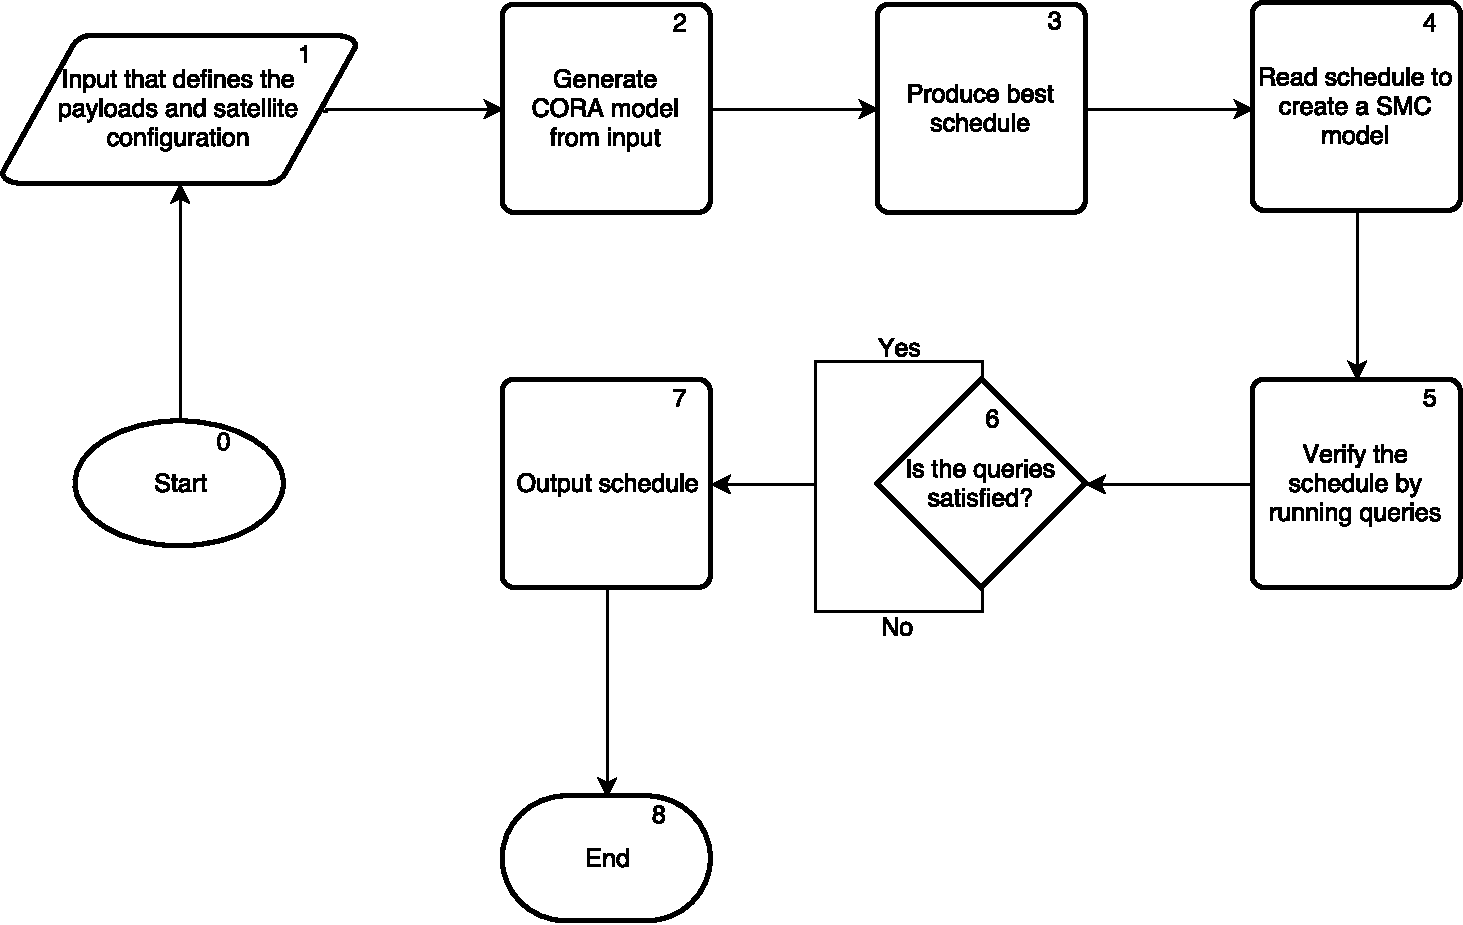
\includegraphics[width=\textwidth]{graphics/flow_act.pdf}
	\caption{Flowchart that displays the actual workflow}
	\label{fig:tool_act}
\end{figure}

\subsection{Battery Wear and Lifetime} \label{subsec:disc_life}
We did not implement any major features that would try to avoid straining the battery. 
But as Wognsen et al. 2015\cite{score_function} expresses, it is important to predict the battery wear for battery powered systems as it is a central part of predicting the system's lifetime.
The major reason for why no such features were implemented, where that it was difficult to find a balance between not wearing the battery and executing payloads.
Wognsen et al. 2015\cite{score_function} presented a scoring function to compare and evaluate the impact of battery usage profiles on cycle life. Their scoring system would have been simple to implement as the \gls{cora} model is always aware of the battery's \gls{soc}. However, the authors conclude that the score does not indicate to what effect the usage profile will have on the battery life. They do note that it is expected that with a large enough amount of experiment data, it would be possible to tailor the function to a specific battery type, such as the one that GomX-3 is equipped with. We were not interested in obtaining this data as we found other problems more pressing during the duration of the project.\\
It is difficult to use the scoring system without knowing what the scores represent in actual wear, as it makes it hard to determine 


We are currently not able to model that the battery deteriorate over time, but since the user can theoretically calculate the actual capacity of the battery and set the maximum capacity to that value, it is possible to pass the information to the model.

However, a location have been added to the UPPAAL \gls{smc} model in order to avoid overcharging the battery, as explained in \myref{sec:smc_model}.\\

We believe that since our tool has an emphasis on battery usage, the ability to model battery wear and avoid schedules that have a high impact on it, will be sensible to implement. 

\subsection*{Improving Insolation}
As mentioned in \myref{sec:cora} the model always assume an initial state of insolation, that the nanosatellite is in the sun. Resulting in our schedule only being able to generate schedules for the nanosatellite when it matches our starting point.
This could be corrected by adding new initial location, that have transitions to both of the existing locations, given a variable that will determine which location there should be transitioned to based on the actual position of the satellite.


\subsection*{Zero Windows}
As of now the models, both \gls{cora} and \gls{smc}, does not support there being no defined windows in the payload description as several variables are dependant on this. However, as windows is an important concept for our context we do not believe this to be a problem. Also there is a workaround by defining all payloads as having the window $0-OrbitTime$.

\subsection*{Battery Importance}
During our meeting with Lars Alminde at GomSpace we discussed our approach as well as potential new approaches. They expressed that nanosatellites battery was not as important as we had initial assumed\cite{gom_space_conversation}. this may be a combination of multiple factors like increased battery capacity and more efficient solar panels. Given that our meeting with GomSpace was late in the project we decided to keep battery as an aspect of our problem statement.

\section{Inaccuracies and Assumptions}\label{sec:in_and_ass}
During our development of the \gls{cora} and \gls{smc} models, we have made some decisions which may not always be an accurate representation of the outside world. In this section we will discuss each of these choices to evaluate the potential effect, these inaccuracies and assumptions may have on the produced schedule.

%More than one window for a payload \cref{ssec:multi_window}
In \myref{sec:read_input} we describe how a payload can have an associated window in which the payload can be executed, but the possibility of a payload having multiple windows was never explored, despite of our models supporting it. Unfortunately our payload descriptions semantics does not allow for multiple windows. This has the potential to make the produced schedule differ significantly from the actually optimal schedule, and we therefore believe this to be a significant inaccuracy.

Introducing the variable idle\_cost to our \myref{sec:read_input} could reduce the computation time required for producing a schedule in \gls{cora}. It is meant to reduce the number of payloads, by removing operational payloads that run frequently and adds no profit to the schedule. And simulate their energy requirements via the idle\_cost variable. But this could give misleading results since idle\_cost represent the average energy cost for the operational payloads and continuously drain on the battery unlike payloads that only drains on the battery for short periods. But by setting idle\_cost to zero and specifying all payload running on the nanosatellite this variable will not cause any misrepresentation to the produced schedule.

In \myref{sec:cora} we mention the need for priorities to indicate the profit for each of the payloads, the prioritisation can be set to a value between zero and five, five being the most important payload to execute in terms of profit. This dose not immediately impose any inaccuracies unless the user defines more than six payloads each with their distinct priority.

We used an Ideal battery model given \gls{cora} restrictions, This will according to the observations made during \myref{sec:kibam} overestimate the battery compared to a real battery, which produces schedules that uses more energy than they have. The impact of this is mitigated with our \gls{smc} model having a more pessimistic battery model.

The Processor template in the \gls{cora} model, see \myref{sec:cora}, models the nanosatellite's processor. Here we mentions two factor that can have an effect on the optimal schedule. A payload is always executed based on its worst execution time, and deadlines force the model to wait a period after the payload has been executed. Payloads running worst case has the benefit of taken more energy from a battery model that already overestimate the actual value. But schedules produced this way may sometimes be less profitable, compared to schedules generate based on best case running time for payloads, the drawback with this approach is the reduced energy taken from the battery and potentially skipping payloads due to some payloads taking a bit more time then the best case and thus causing more energy to be drawn from the battery. This can cause a chain reaction of payloads being skipped based on the individual payloads dependencies and windows when the schedule is verified via \gls{smc}. Additionally the way dependencies are modelled, would not enable all forms of payload dependencies, which can lead to less optimal schedules if user is not able model their payload dependencies with our dependency rules.
Deadlines is only a problem if changes are made to the \gls{cora} model to execute payload in best execution time instead of worst case execution time, because it is possible to set deadline for each payload to their worst case execution time, negating any effect deadlines may have on the schedule. Deadlines are intended to allow payloads in \gls{smc} model to be executed, even when their starting time have passed, as long as it is does not exceed the deadline defined by the payload being executed.

In \gls{cora} \cref{ssec:cora_ins} describing insolation we made two inaccuracies for the sake of performance.  Dividing the number of updates made to the battery during an orbit, and insolation period lasting precisely half the orbit length. Determining the severity of reducing the number of updates to the battery during an orbit, showed a big decrease in time taking to produce the schedule with the effect of an added inaccuracy which we concluded to be neglectable. Another side effect that may occurred  if the orbit length divided by the number of updates produces a fractional number, resulting in \gls{cora} model not updating the correct amount of times for an orbit, due to \gls{cora} rounding down decimals to the nearest natural number.

The PayloadWindow in \myref{sec:cora} mentions that our orbit are modelled circular, where a more representative picture of and orbit would be more oval in shape. This inaccuracy mean that schedules should be rather short in length, because longer schedules further increase the inaccuracy as time goes by.

Modifications to the \gls{smc} model were also been done, as described in \myref{sec:smc_model}, \gls{kibam} is one of the factors that impact the \gls{smc} model, unlike in \gls{cora} where the battery model overestimated the battery, \gls{kibam} underestimate resulting in few schedules being discarded even though the may be viable.

%Starting value from future work \cref{ssec:start_val}
Our \gls{cora} model does not support knowledge from previous schedules, so the variable \uppVar{runs[]} that keep track of which payloads has been executed will always be initialized to zero, making it impossible to generate a schedule based on the \uppVar{runs[]} from the previous schedule.

To conclude on this we can divide the behaviours into two categories, "will", and "may" effect schedule. will includes battery models, worst payload running time, general insolation because these factors will always have an effect on the produced schedule. May on the other hand can be tweaked by the user to have no effect on the produced schedule, these are number of updates per orbit on the battery, five prioritisation limit on payloads, deadline on payloads.
\jfx{Too short? What can we then say?}



 







